\documentclass{beamer}

\usepackage[brazil]{babel}
\usepackage[utf8]{inputenc}
\usepackage[T1]{fontenc}

\usetheme{Madrid}
\setbeamertemplate{navigation symbols}{}

\title[Lógica Computacional]{Lógica Computacional}

\author[Diego S. C. Nascimento]{Diego Silveira Costa Nascimento}

\institute[IFRN]{
Instituto Federal de Educação, Ciência e Tecnologia do Rio Grande do Norte\\
diego.nascimento@ifrn.edu.br
}

\date[\today]{\today}

\begin{document}

\begin{frame}[plain]
	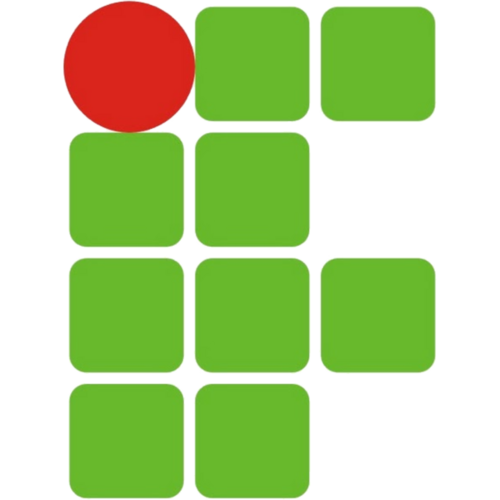
\includegraphics[scale=0.2]{img/IFRN}
	\titlepage
\end{frame}

\logo{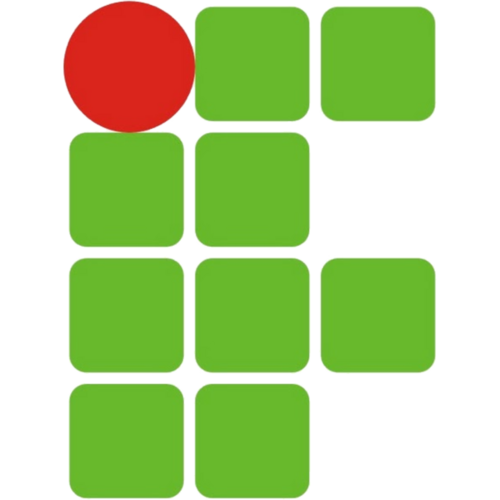
\includegraphics[scale=0.1]{img/IFRN}}

\begin{frame}
	\frametitle{Ementa do Curso}
  	\tableofcontents
\end{frame}

\AtBeginSection[]{
	\begin{frame}
		\frametitle{Ementa do Curso}
		\tableofcontents[currentsection]
	\end{frame}
}

\section{Introdução}

\begin{frame}
	\frametitle{Lógica}

	\begin{block}{Definição}
		É a ciência das leis ideais do pensamento e a arte de aplicá-las à pesquisa e à demonstração da verdade.
	\end{block}\vfill
	
	\begin{itemize}
		\item Deriva do Grego (logos); e
		\item Significa:
			\begin{itemize}
			\item palavra;
			\item pensamento;
			\item ideia;
			\item argumento;
			\item relato;
			\item razão
			\item lógica; ou
			\item princípio lógico.
			\end{itemize}
	\end{itemize}
\end{frame}

\begin{frame}
\frametitle{Origem}

\begin{itemize}
	\item A Lógica teve início na Grécia em 342 a.C.;
	\item Aristóteles sistematizou os conhecimentos existentes em Lógica, elevando-a à categoria de ciência;
	\item Obra chamada Organon (Ferramenta para o correto pensar);
	\item Aristóteles preocupava-se com as formas de raciocínio que, a partir de conhecimentos considerados verdadeiros, permitiam obter novos conhecimentos; e
	\item A partir dos conhecimentos tidos como verdadeiros, caberia à Lógica a formulação de leis gerais de encadeamentos lógicos que levariam à descoberta de novas verdades.
\end{itemize}\vfill

\begin{columns}[c] 
	\column{.3\textwidth}
	\begin{exampleblock}{Aristóteles}
		\center
		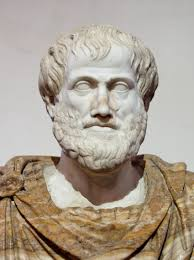
\includegraphics[scale=0.18]{img/aristoteles}
	\end{exampleblock}
	
	\column{.3\textwidth}
	\begin{exampleblock}{Organon}
		\center
		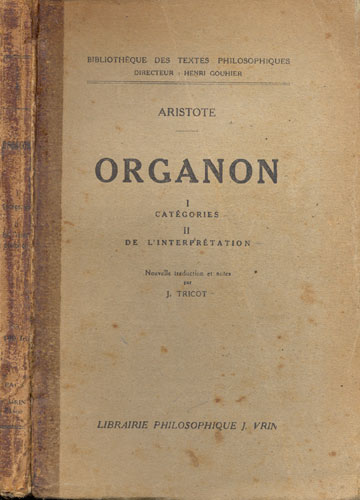
\includegraphics[scale=0.1]{img/organon}	
	\end{exampleblock}
	
\end{columns}
\end{frame}

\begin{frame}
\frametitle{Princípios Lógico}

A Lógica Formal repousa sobre três princípios fundamentais que permitem todo seu desenvolvimento posterior, e que dão validade a todos os atos do
pensamento e do raciocínio.

\begin{exampleblock}{Princípio da Identidade}
Afirma $A = A$ e não pode ser $B$, o que é, é.
\end{exampleblock}\vfill
	
\begin{exampleblock}{Princípio da Não Contradição}
$A = A$ e nunca pode ser não-$A$, o que é, é e não pode ser sua negação, ou seja, o ser é, o não ser não é.
\end{exampleblock}\vfill

\begin{exampleblock}{Princípio do Terceiro Excluído}
Afirma que Ou $A$ é $x$ ou $A$ é $y$, não existe uma terceira possibilidade.
\end{exampleblock}

\end{frame}

\end{document}